\documentclass[10pt,a4paper]{article}

\usepackage{graphicx}
\usepackage{amsmath}
\usepackage{amsfonts}
\usepackage{amssymb}


\usepackage[T2A]{fontenc}
\usepackage[utf8]{inputenc}
\usepackage[ukrainian]{babel} 

\numberwithin{figure}{section}
\numberwithin{equation}{section}

\title{Амплітудно-частотні характеристики шаруватих пластин і циліндричних оболонок зі складною геометрією напрямної}
\author{{\large Горячко Тарас Всеволодович}\\[10mm] Науковий керівник: доктор фізико-математичних наук, професор\\ Марчук М.В. }
\date{}
\begin{document}
\maketitle

Шановний пане голово, шановні члени вченої ради та опоненти!\\

До Вашої уваги пропонується доповідь за матеріалами дисертаційної роботи на здобуття наукового ступення кандидата фізико-математичних наук (за спеціальністю………???? – не знаю чи потрібно) на тему \textbf{«Амплітудно-частотні характеристики шаруватих пластин і циліндричних оболонок зі складною геометрією напрямної»}.\\

\section*{Вступ}
У вступі обґрунтовано актуальність теми дисертації, відзначено зв’язок роботи з науковими темами і програмами, сформульовано \textbf{мету}, якою є \textit{«Розвиток методу збурень в поєднанні з методом скінченних елементів стосовно задач визначення амплітудно-частотних характеристик шаруватих пластин і циліндричних оболонок з складною геометрією напрямної за лінійних та геометрично  нелінійних коливань»} і завдання досліджень,  висвітлено наукову новизну, наукове та практичне значення, обґрунтовано достовірність отриманих результатів. Зазначено \textbf{об’єкт дослідження}, яким є \textit{«Процеси лінійних і геометрично нелінійних коливань шаруватих пластин і циліндричних оболонок зі складною геометрією напрямної»}, та названо \textbf{предмет досліджень} --- \textit{«Спектри власних частот та амплітудно-частотні залежності шаруватих пластин і циліндричних оболонок зі складною геометрією напрямної за лінійних та геометрично  нелінійних коливань»}. Наведено дані про апробацію отриманих результатів, виокремлено особистий внесок дисертанта у публікаціях, підготовлених за участю співавторів, а також наведено відомості про структуру та об’єм (обсяг) роботи. 
\section{Розділ 1}
У першому розділі за літературними джерелами проаналізовано \textit{«Основні методи і результати теоретичних досліджень за проблемою визначення  амплітудно-частотних характеристики шаруватих пластин і циліндричних оболонок за лінійного та геометрично нелінійного деформування.»}

\medskip 
\textbf{Огляд публікацій за проблемою теоретичного аналізу лінійних і нелінійних коливань оболонок і пластин}

\medskip 
Дослідження процесів лінійних та нелінійних коливань тонкостінних елементів конструкцій із традиційних матеріалів було започатковано на основі використання класичної теорії, що базується на гіпотезі Кірхгофа-Лява. Фундаментальні результати в цьому напрямку отримані в працях  В.В. Болотіна, А.С. Вольміра, В.Т. Грінченка, Я.М. Григоренка, В.А. Криська, В.Д. Кубенка, Л.В. Курпи, С.П. Тимошенка та інших учених. 

\medskip 
Слід відмітити, що такий підхід дозволяє врахувати анізотропію фізико-механічних характеристик лише в тангенціальних напрямках, однак, не дозволяє дослідити вплив на амплітудно частотні характеристики  таких специфічних властивостей нових матеріалів - композитів, як податливість до трансверсальних зсуву та стиснення.

\medskip Суттєві результати у вирішенні цієї проблеми містяться в роботах І. Альтенбаха, С.О. Амбарцумяна, І.М. Векуа, К.З. Галімова, Я.М. Григоренка, О.М. Гузя, В.С. Гудрамовича, Р. Міндліна, П. Нагді, Ю.В. Немировського, Б.Л Пелеха, В.Г. Піскунова, Е. Рейснера, М.А. Сухорольського, В.П. Тамужа, С.П. Тимошенка, Л.П. Хорошуна та інших учених.
\medskip 

Дія інтенсивних динамічних (зокрема циклічних) експлуатаційних навантажень спричиняє поперечні переміщення в тонкостінних елементах, котрі співмірні з їхніми товщинами. Це зумовлює геометрично нелінійний характер їх деформованого стану. 
\medskip 

Постановкам задач про лінійній та геометрично нелінійні коливання пластин і оболонок та розробці методів їх розв'язання на основі застосування уточнених теорій присвячені праці О.І. Беспалової, В.В. Болотіна, А.С. Вольміра, В.Т. Грінченка, О.Я. Григоренка, Я.М. Григоренка, В.А. Криська, Л.В. Курпи, М.В. Марчука, Я.Г. Савули, В.І. Сторожева, С.П. Тимошенка, M. Amabili, J Awrejcewicz, I.K. Banerjee, I.C. Chen, Li. A. Dong, C.L. Dym, D.A. Evenren, P.B. Goncalves, E.L. Jansen, L. Librescu, F.M.A. Silva, M. Sundhakar, T. Ueda та інших учених.
\medskip 

Дослідження коливних процесів тонкостінних елементів на основі просторових співвідношень динамічної теорії пружності відображенні ????Альтенбах Е. В. Алтухова [3–4], И.И. Воровича, С. Г. Лехницкого, Л. С. Плевако, А. К. Приварникова, Р. М. Раппопорт, А. О. Рассказова, В. И. Сторожева [58], Ю. А. Устинова, В.А. Шалдырвана [23] и др

\medskip 
Розробці та розвиненню методів розв'язування результуючих систем  нелінійних алгебнаїчних рівнянь присвячені роботи Бате,

\section{Розділ 2. РІВНЯННЯ ДИНАМІЧНО НАПРУЖЕНОГО СТАНУ ЗА ГЕОМЕТРИЧНО НЕЛІНІЙНОГО ДЕФОРМУВАННЯ}

У другому розділі спочатку наведено «рівняння динамічно напруженого стану за геометрично нелінійного деформування»

\subsection{Співвідношення просторової геометрично нелінійної динамічної теорії пружності в криволінійній системі координат
}

\begin{figure}
\begin{center}
			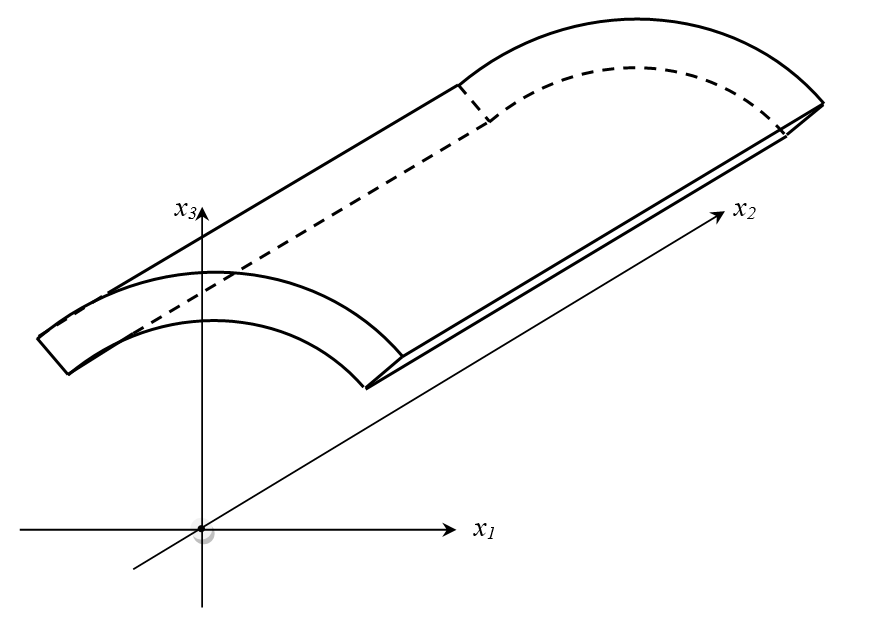
\includegraphics[scale=0.3]{pic/layer.png}			\end{center}
			\caption{Криволінійний пружний шар у декартовій системі координат}
			\label{fig:21}
		\end{figure}
		

\begin{align}
\vec{u} &= u^i \vec{R_i}=u_i \vec{R^i} \label{eq:u_v}\\
\hat{\varepsilon} &= \varepsilon^{ij} \vec{R_i}\vec{R_j}=\varepsilon_{ij} \vec{R^i}\vec{R^j} \label{eq:stran_t}\\
\hat{\Sigma} &= \sigma^{ij} \vec{R_i}\vec{R_j}=\sigma_{ij} \vec{R^i}\vec{R^j} \label{eq:stress_t}\\
\varepsilon_{ij} &= \frac{1}{2} \left( \nabla_i u_j + \nabla_j u_i + \nabla_i u^j \nabla_j u_k \right) \label{eq:stran_to_u}\\
\nabla_j u_i &= \frac{ \partial u_i }{ \partial \alpha_j } - u_k G ^k _{ij} \label{eq:du} \\
G ^k _{ij} &= \frac12 \sum_{m=1}^{3} g^{km} 
\left(
\frac{\partial g_{im}}{\partial \alpha_j} + \frac{\partial g_{jm}}{\partial \alpha_i} - \frac{\partial g_{ij}}{\partial \alpha_m} 
\right) \label{eq:sK} \\
\sigma^{ij} &= C^{ijkm}\varepsilon^{km} \label{eq:hook_law}
\end{align}

Для цього розглянуто криволінійний шар рисунок \ref{fig:21}. Його напружено-деформований стан описується вектором просторовий переміщень \eqref{eq:u_v}, тензором деформацій \eqref{eq:stran_t} і тензором напружень Коші \eqref{eq:stress_t}. Зв’язок між компонентами вказаних об’єктів визначається деформаційними співвідношеннями \eqref{eq:stran_to_u} з урахуванням \eqref{eq:du}, \eqref{eq:sK} і співвідношеннями пружності (узагальненим законом Гука) \eqref{eq:hook_law}.

\emph{Рівняння руху точок шару} мають вигляд \eqref{eq:P}
\begin{equation} \label{eq:P}
div \hat{P} = \rho \frac{\partial^2 \vec{u}}{\partial t^2},
\end{equation}
де $\hat{P}$ --- перший несиметричний тензор Кірхгофа-Піоли, $\rho$ --- густина, $t$ --- час.

\medskip
Для однозначного інтегрування  \eqref{eq:P} необхідно записати граничні умови на поверхні шару та описати конфігурацію, яку займає шар в початковий момент часу. На лицевих поверхнях шару граничні умови записано у вигляді 
\begin{equation}
P^{3i}\left( \alpha_1, \alpha_2, \pm \frac{h}{2}, t \right) = X^{\pm}_{3i}\left( \alpha_1, \alpha_2, t \right).
\end{equation}

\medskip
На боковій поверхні $\Omega$, яка складається з двох частин, на одній з яких задані переміщення $\Omega_{u} $, а на іншій – зовнішні зусилля $\Omega_{\sigma} $, граничні умови подано у вигляді  
\begin{align}
P^{im}\left( \alpha_1, \alpha_2, \alpha_3, t \right)n_i &= f^{m}\left( \alpha_1, \alpha_2, \alpha_3, t \right), i=1,2,3, m=1,2,3, \left( \alpha_1, \alpha_2,\alpha_3\right)\in\Omega_{\sigma};\\
u^{i}\left( \alpha_1, \alpha_2, \alpha_3, t \right) &=g^{i}\left( \alpha_1, \alpha_2, \alpha_3, t \right), i=1,2,3, \left( \alpha_1, \alpha_2,\alpha_3\right)\in\Omega_{u}.
\end{align}

\emph{Початкові умови}
\begin{equation}
u^{i}\vline _{t=t_0} = u^i_0 \left( \alpha_1, \alpha_2, \alpha_3 \right); \frac{\partial u^{i}}{\partial t}\vline _{t=t_0} =v^i_0 \left( \alpha_1, \alpha_2, \alpha_3 \right); i=1,2,3.
\end{equation}

\textbf{2.2. Варіаційна постановка задачі}
\begin{equation}
\int_{V(t)} \delta\hat{E}:\hat{\tau}\,dV+\int_{V(t)} \rho \delta\vec{u} \frac{\partial^2 \vec{u}}{\partial t ^2}\,dV=\int_{\Omega_\sigma(t)} \delta\vec{u} \vec{f} \,dS
\end{equation}

\[
\forall \delta\vec{u} \in D_A 
= \{ 
\vec{u}:\vec{u}\in W_2^{(2)}; 
\vec{u}=\vec{g} \left( \alpha_1, \alpha_2,\alpha_3 \right) \in \Omega_{u}, \forall t \}
\]

\begin{tabbing}
де \= $ W_2^{(2)}$ --- простір Соболєва,\\
\> $\hat{\tau}$ --- тензор напружень Коші,\\
\> $\vec{f}$ --- вектор поверхневих сил,\\
\> $\delta\hat{E}$ --- тензор лінійних деформацій, який відповідає варіації переміщень.
\end{tabbing}
Оскільки $V(t)$ є невідомим, то в початковій (недеформованій) конфігурації:
\begin{equation}\label{eq:virtwork_gen}
\int_{V_0} \delta\hat{\varepsilon}:\hat{S}\,dV+\int_{V_0} \rho_0 \delta\vec{u} \frac{\partial^2 \vec{u}}{\partial t ^2}\,dV=\int_{\Omega_{\sigma0}} \delta\vec{u} \vec{f} \,dS
\end{equation}

\begin{tabbing}
де \= $\hat{S}$ --- другий симетричний тензор напружень Кірхгофа-Піоли, \\для якого справедлива формула $\hat{S} = \hat{P} \left( \hat{F}^{-1} \right)^T $,\\
\> $\hat{P}$ --- тензор з формули \ref{eq:P},\\
\> $\hat{F}=\hat{G} + grad^T \vec{u}$ --- тензор градієнта локального руху,\\
\> $\delta\hat{\varepsilon}$ --- тензор деформацій Гріна, який відповідає варіації переміщень.
\end{tabbing}


\textbf{2.3. Компоненти тензора деформацій в довільній системі координат}
\begin{equation}
\vec{\nabla} \vec{u} =  
B \cdot \tilde{u}
\end{equation}
де \\
\begin{equation}
\vec{\nabla} \vec{u} =  \left(
\nabla_1 u_1  \nabla_2 u_1  \nabla_3 u_1 \nabla_1 u_2  \nabla_2 u_2  \nabla_3 u_2 
\nabla_1 u_3  \nabla_2 u_3  \nabla_3 u_3 
\right)^T
\end{equation}
\begin{equation}
 \tilde{u} =  \left( u_1 
\frac { \partial u_1 } { \partial \alpha_1} 
\frac { \partial u_1 } { \partial \alpha_2} 
\frac { \partial u_1 } { \partial \alpha_3} 
u_2 
\frac { \partial u_2 } { \partial \alpha_1} 
\frac { \partial u_2 } { \partial \alpha_2} 
\frac { \partial u_2 } { \partial \alpha_3} 
u_3 
\frac { \partial u_3 } { \partial \alpha_1} 
\frac { \partial u_3 } { \partial \alpha_2} 
\frac { \partial u_3 } { \partial \alpha_3} 
\right)^T
\end{equation}
матриця $B$:
\begin{equation}\label{eq:matrixB}
B=
\left[\begin{array}{cccccccccccc}
-G_{11}^1 & 1 & 0 & 0 & -G_{11}^2 & 0 & 0 & 0 & -G_{11}^3 & 0 & 0 & 0\\
-G_{12}^1 & 0 & 1 & 0 & -G_{12}^2 & 0 & 0 & 0 & -G_{12}^3 & 0 & 0 & 0\\
-G_{13}^1 & 0 & 0 & 1 & -G_{13}^2 & 0 & 0 & 0 & -G_{13}^3 & 0 & 0 & 0\\
-G_{21}^1 & 0 & 0 & 0 & -G_{21}^2 & 1 & 0 & 0 & -G_{21}^3 & 0 & 0 & 0\\
-G_{22}^1 & 0 & 0 & 0 & -G_{22}^2 & 0 & 1 & 0 & -G_{22}^3 & 0 & 0 & 0\\
-G_{23}^1 & 0 & 0 & 0 & -G_{23}^2 & 0 & 0 & 1 & -G_{23}^3 & 0 & 0 & 0\\
-G_{31}^1 & 0 & 0 & 0 & -G_{31}^2 & 0 & 0 & 0 & -G_{31}^3 & 1 & 0 & 0\\
-G_{32}^1 & 0 & 0 & 0 & -G_{32}^2 & 0 & 0 & 0 & -G_{32}^3 & 0 & 1 & 0\\
-G_{33}^1 & 0 & 0 & 0 & -G_{33}^2 & 0 & 0 & 0 & -G_{33}^3 & 0 & 0 & 1
\end{array}\right]
\end{equation}

Формула для компонент тензора деформацій Гріна
\begin{equation}
\vec{\varepsilon}=\vec{e}+\vec{\eta}=\left(E + E_{NL}^{(1)} \left(\vec {\nabla} \vec{u} \right) \right)\vec {\nabla} \vec{u}=\left(E + E_{NL}^{(2)} \left(\vec {\nabla} \vec{u} \right) \right)\vec {\nabla} \vec{u}
\end{equation}
де 
\begin{align}
\vec{\varepsilon} = \left(
\varepsilon_{11}\,
\varepsilon_{22}\,
\varepsilon_{33}\,
2\varepsilon_{12}\,
2\varepsilon_{13}\,
2\varepsilon_{23}\,
\right)^T,\\
\vec{e} = \left( 
e_{11}\,
e_{22}\,
e_{33}\,
2e_{12}\,
2e_{13}\,
2e_{23}\,
\right)^T,\\
\vec{\eta} = \left( 
\eta_{11}\,
\eta_{22}\,
\eta_{33}\,
2\eta_{12}\,
2\eta_{13}\,
2\eta_{23}\,
\right)^T,
\end{align}
матриця $E$:
\begin{equation}
E=\left[\begin{matrix}1 & 0 & 0 & 0 & 0 & 0 & 0 & 0 & 0\\0 & 0 & 0 & 0 & 1 & 0 & 0 & 0 & 0\\0 & 0 & 0 & 0 & 0 & 0 & 0 & 0 & 1\\0 & 1 & 0 & 1 & 0 & 0 & 0 & 0 & 0\\0 & 0 & 1 & 0 & 0 & 0 & 1 & 0 & 0\\0 & 0 & 0 & 0 & 0 & 1 & 0 & 1 & 0\end{matrix}\right],
\end{equation}


матриці $E_{NL}^{(1)}, E_{NL}^{(2)}$:
\begin{equation}
E_{NL}^{(1)}=\left[\begin{matrix}
\frac{\lambda_{11}}{2} & 0 & 0 & \frac{\lambda_{21}}{2} & 0 & 0 & \frac{\lambda_{31}}{2} & 0 & 0\\
0 & \frac{\lambda_{12}}{2} & 0 & 0 & \frac{\lambda_{22}}{2} & 0 & 0 & \frac{\lambda_{32}}{2} & 0\\
0 & 0 & \frac{\lambda_{13}}{2} & 0 & 0 & \frac{\lambda_{23}}{2} & 0 & 0 & \frac{\lambda_{33}}{2}\\
0 & \lambda_{11} & 0 & 0 & \lambda_{21} & 0 & 0 & \lambda_{31} & 0\\
\lambda_{13} & 0 & 0 & \lambda_{23} & 0 & 0 & \lambda_{33} & 0 & 0\\
0 & 0 & \lambda_{12} & 0 & 0 & \lambda_{22} & 0 & 0 & \lambda_{32}
\end{matrix}\right],
\end{equation}
\begin{equation}
E_{NL}^{(2)}=\left[\begin{matrix}
\frac{\lambda_{11}}{2} & 0 & 0 & \frac{\lambda_{21}}{2} & 0 & 0 & \frac{\lambda_{31}}{2} & 0 & 0\\
0 & \frac{\lambda_{12}}{2} & 0 & 0 & \frac{\lambda_{22}}{2} & 0 & 0 & \frac{\lambda_{32}}{2} & 0\\
0 & 0 & \frac{\lambda_{13}}{2} & 0 & 0 & \frac{\lambda_{23}}{2} & 0 & 0 & \frac{\lambda_{33}}{2}\\
\lambda_{12} & 0 & 0 & \lambda_{22} & 0 & 0 & \lambda_{32} & 0 & 0\\
0 & 0 & \lambda_{11} & 0 & 0 & \lambda_{21} & 0 & 0 & \lambda_{31}\\
0 & \lambda_{13} & 0 & 0 & \lambda_{23} & 0 & 0 & \lambda_{33} & 0
\end{matrix}\right],
\end{equation}
де
$ \lambda_{ij}=\sum_k g^{ik}\nabla_j u_k $.

\textbf{2.4. Фізичні компоненти переміщень і параметри Ламе}
\linebreak
\linebreak
Змішана криволінійна ортогональна система координат:
\begin{align}
g_{11}=H_1^2; g_{22}=H_2^2; g_{33}=1; \\
g_{ij}=0; i,j=1,2,3, i \ne j;
\end{align}
Довільна циліндрична система координат
\begin{align}
H_1 = H_1 \left( \alpha_1, \alpha_2, \alpha_3 \right) &= A \left( \alpha_1 \right) \left( 1+ \alpha_3 K \left( \alpha_1 \right) \right)  \\
H_2 = H_2 \left( \alpha_1, \alpha_2, \alpha_3 \right) &= 1
\end{align}

\begin{tabbing}
де \= $  A \left( \alpha_1 \right)$ --- коефіцієнт першої квадратичної форми серединної поверхні оболонки,\\
\> $K \left( \alpha_1 \right)$ --- головна кривина напрямної??? в напрямку осі $\alpha_1$.
\end{tabbing}
тоді матриця $B$ \eqref{eq:matrixB}
\begin{equation}
\begin{aligned}
B=
\left[\begin{array}{@{}c@{\hspace{-8pt}}c@{\hspace{2pt}}ccc@{\hspace{2pt}}c@{\hspace{2pt}}cc@{\hspace{1pt}}c@{\hspace{-8pt}}c@{\hspace{1pt}}cc}
0 & \frac{1}{A \left(1+ \alpha_{3} K \right)} & 0 & 0 & 0 & 0 & 0 & 0 & \frac{K}{1+ \alpha_{3} K } & 0 & 0 & 0\\0 & 0 & 1 & 0 & 0 & 0 & 0 & 0 & 0 & 0 & 0 & 0\\0 & 0 & 0 & 1 & 0 & 0 & 0 & 0 & 0 & 0 & 0 & 0\\0 & 0 & 0 & 0 & 0 & \frac{1}{A \left(1+ \alpha_{3} K \right)} & 0 & 0 & 0 & 0 & 0 & 0\\0 & 0 & 0 & 0 & 0 & 0 & 1 & 0 & 0 & 0 & 0 & 0\\0 & 0 & 0 & 0 & 0 & 0 & 0 & 1 & 0 & 0 & 0 & 0\\- \frac{K}{1+ \alpha_{3} K } & 0 & 0 & 0 & 0 & 0 & 0 & 0 & 0 & \frac{1}{A \left(1+ \alpha_{3} K \right)} & 0 & 0\\0 & 0 & 0 & 0 & 0 & 0 & 0 & 0 & 0 & 0 & 1 & 0\\0 & 0 & 0 & 0 & 0 & 0 & 0 & 0 & 0 & 0 & 0 & 1\end{array}\right]
\end{aligned}
\end{equation}


\textbf{2.5. Варіаційна постановка задачі відносно переміщень.}
\begin{align}
\int_{V_0} \delta\hat{\varepsilon}:\hat{S}\,dV=\int_{V_0} \delta\overline{u} ^T B ^T\left( E + E_{NL} \right)^T C \left( E + E_{NL}^{(1)} \right)B \overline{u} \, dV\\ \int_{V_0} \rho_0 \delta\tilde{u} ^T \frac{\partial^2 \tilde{u}}{\partial t ^2}\,dV=\int_{V_0} \rho_0 \delta\overline{u} ^T \tilde{B}^T \tilde{B}\frac{\partial^2 \overline{u}}{\partial t ^2}\,dV
\end{align}
Тоді \eqref{eq:virtwork_gen}:
\begin{multline} \label{eq:virtwork_gen_u}
\int_{V_0} \delta\overline{u} ^T B ^T\left( E + E_{NL} \right)^T C \left( E + E_{NL}^{(1)} \right)B \overline{u} \, dV+\\+\int_{V_0} \rho_0 \delta\overline{u} ^T \tilde{B}^T \tilde{B}\frac{\partial^2 \overline{u}}{\partial t ^2}\,dV=F_{out}
\end{multline}


\textbf{2.6. Побудова одновимірної моделі на основі двовимірної.}
\linebreak
\linebreak
Апроксимація переміщень $u_1$ та $u_3$, за координатою $\alpha_3$ 
\begin{align}
u_1 \left( \alpha_1, \alpha_3 \right) = u_{10} \left( \alpha_1\right)p_0 \left( \alpha_3\right)+u_{11} \left( \alpha_1\right)p_1 \left( \alpha_3\right)+u_{12} \left( \alpha_1\right)p_2 \left( \alpha_3\right),\\
u_3 \left( \alpha_1, \alpha_3 \right) = u_{30} \left( \alpha_1\right)p_0 \left( \alpha_3\right)+u_{31} \left( \alpha_1\right)p_1 \left( \alpha_3\right)+u_{32} \left( \alpha_1\right)p_2 \left( \alpha_3\right),
\end{align}
де поліноми $p_0$, $p_1$ та $p_2$ мають вигляд
\begin{equation}
p_0 \left( \alpha_3\right) = \frac12-\frac{\alpha_3}{h},
p_1 \left( \alpha_3\right) = \frac12+\frac{\alpha_3}{h},
p_2 \left( \alpha_3\right) = 1-\left(\frac{2\alpha_3}{h}\right)^2,
\end{equation}
$h$ --- товщина шару.
\begin{figure}
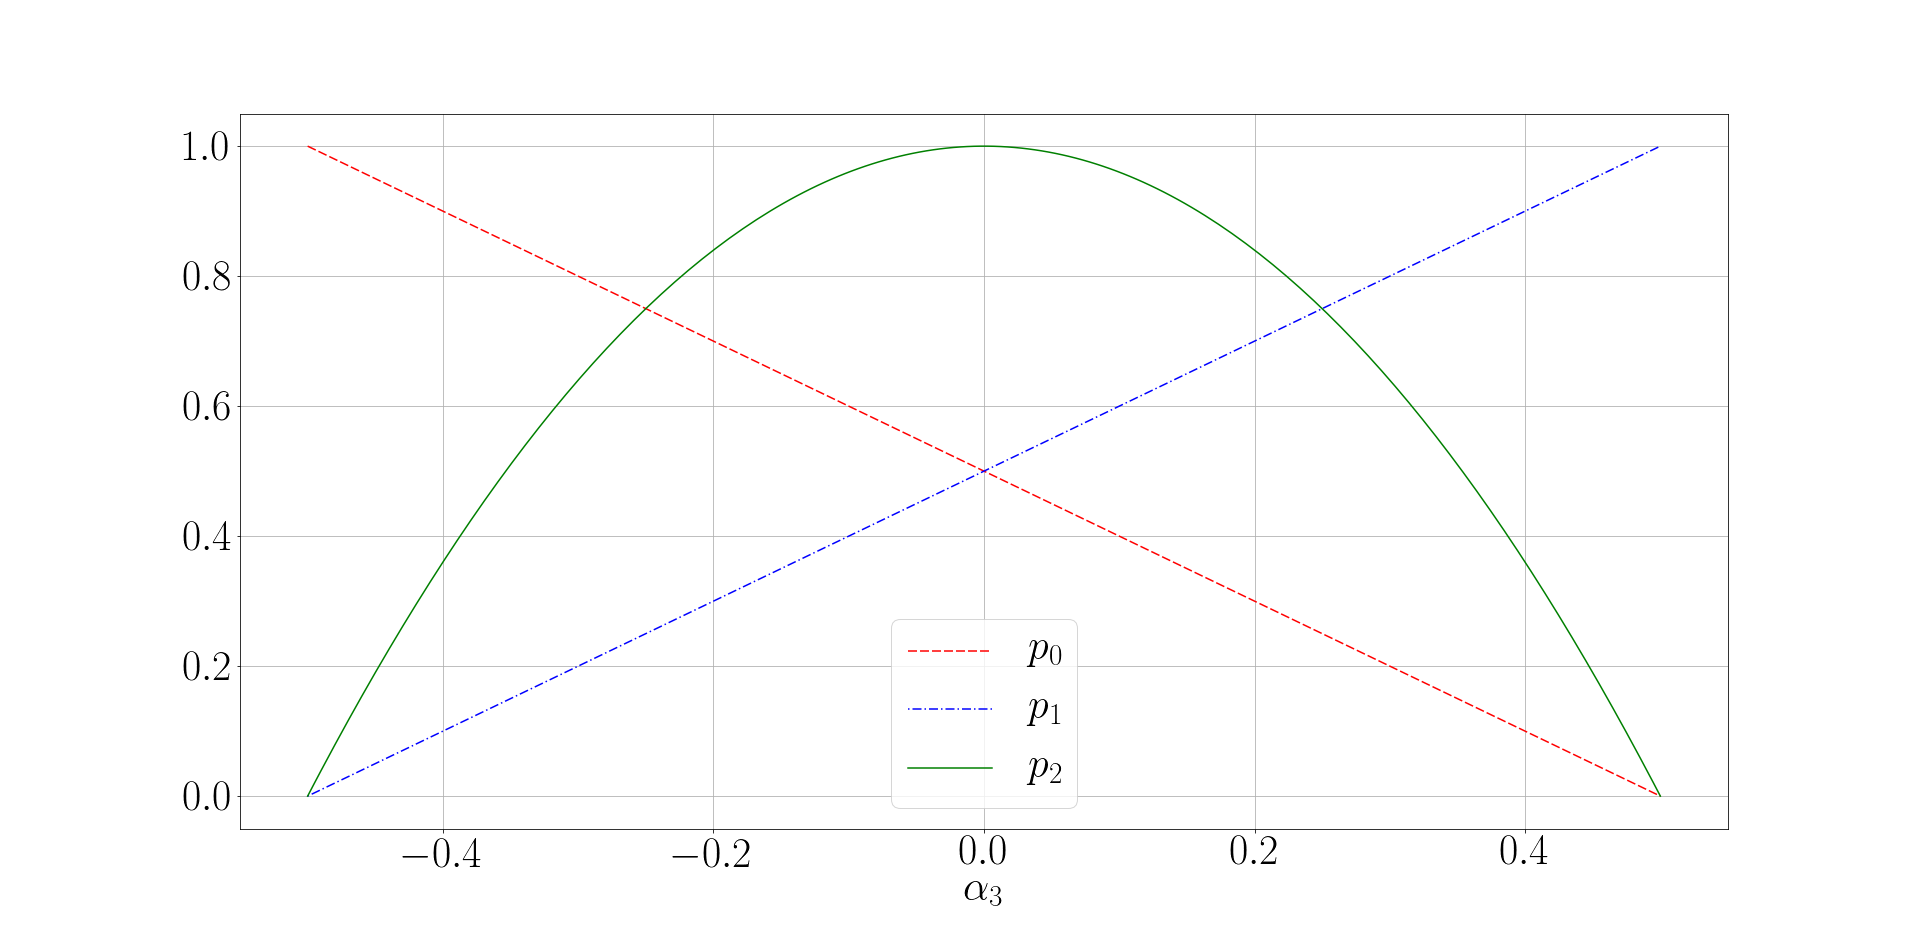
\includegraphics[scale=0.1]{pic/polin.png}
\caption{Графіки поліномів $p_0$, $p_1$ та $p_2$ на проміжку [-0.5;0.5]}
\end{figure}


\begin{equation}
\begin{aligned}
&\varepsilon_{ij} \left( \alpha_1, \alpha_3 \right) = \frac{\varepsilon_{ij0} \left( \alpha_1\right)p_0 \left( \alpha_3\right)+\varepsilon_{ij1} \left( \alpha_1\right)p_1 \left( \alpha_3\right)+\varepsilon_{ij2} \left( \alpha_1\right)p_2 \left( \alpha_3\right)}{1+\alpha_3 K},\\
&\varepsilon_{ijk} = e_{ijk}\left( \alpha_1\right)+\eta_{ijk}\left( \alpha_1\right), \quad i,j=1,3; k=0,1,2
\end{aligned}
\end{equation}

\begin{tabbing}
де \= $e_{ijk}\left( \alpha_1\right)$ --- лінійна складова,\\
\> $\eta_{ijk}\left( \alpha_1\right)$ --- нелінійна складова.
\end{tabbing}


\begin{equation}\label{eq:sqt_strain_l}
\begin{aligned}
&e_{11k}\left(\alpha_1\right)=\frac{1}{A\left(\alpha_1\right)}\frac{du_{1k}}{d\alpha_1}+u_{3k}K\left(\alpha_1\right), k=0,1,2
\\
&\begin{split}
e_{130}\left(\alpha_1\right)=u_{10}\left( -\frac{1}{h}-\frac{K\left( \alpha_1 \right)}{2} \right)+u_{11}\left( \frac{1}{h}-\frac{K\left( \alpha_1 \right)}{2} \right)+ \\ +u_{12}\left( \frac{4}{h}-2K\left( \alpha_1 \right) \right) + \frac{1}{A\left(\alpha_1\right)}\frac{du_{30}}{d\alpha_1}
\end{split}\\
&\begin{split}
e_{131}\left(\alpha_1\right)=u_{10}\left( -\frac{1}{h}-\frac{K\left( \alpha_1 \right)}{2} \right)+u_{11}\left( \frac{1}{h}-\frac{K\left( \alpha_1 \right)}{2} \right)+\\+u_{12}\left( - \frac{4}{h}-2K\left( \alpha_1 \right) \right) + \frac{1}{A\left(\alpha_1\right)}\frac{du_{31}}{d\alpha_1}
\end{split}\\
&e_{132}\left(\alpha_1\right)=\frac{1}{A\left(\alpha_1\right)}\frac{du_{32}}{d\alpha_1}+u_{12}K\left(\alpha_1\right), k=0,1,2\\
&\begin{split}
e_{330}\left(\alpha_1\right)=u_{30}\left( -\frac{1}{h}+\frac{K\left( \alpha_1 \right)}{2} \right)+u_{31}\left( \frac{1}{h}-\frac{K\left( \alpha_1 \right)}{2} \right)+\\+u_{32}\left( \frac{4}{h}-2K\left( \alpha_1 \right) \right)
\end{split}\\
&\begin{split}
e_{331}\left(\alpha_1\right)=u_{30}\left( -\frac{1}{h}-\frac{K\left( \alpha_1 \right)}{2} \right)+u_{31}\left( \frac{1}{h}+\frac{K\left( \alpha_1 \right)}{2} \right)+\\+u_{32}\left( -\frac{4}{h}-2K\left( \alpha_1 \right) \right)
\end{split}\\
&e_{332}\left(\alpha_1\right)=2K\left( \alpha_1 \right)u_{32}
\end{aligned}
\end{equation}

\begin{equation}
\begin{aligned}
&\eta_{iik}\left(\alpha_1\right)=\left[\begin{array}{ccc}
\omega_{20} & \omega_{21} & \omega_{22}
\end{array} \right] \Theta_k\left(\alpha_1\right) \left[\begin{array}{ccc}
\omega_{20} & \omega_{21} & \omega_{22}
\end{array} \right]^T,\\
&\eta_{13k}\left(\alpha_1\right)=0, \quad k=0,1,2, i=1,3
\end{aligned}
\end{equation}
де
\begin{equation}\label{eq:sqt_strain_nl}
\begin{aligned}
\Theta_0\left(\alpha_1\right)=\frac{1}{32}
\left[
\begin{array}{ccc}
16+6Kh+K^2h^2 & 4Kh+2K^2h^2 & 16+16Kh+4K^2h^2 \\ 
4Kh+2K^2h^2 & -2Kh+K^2h^2 & -16Kh+4K^2h^2 \\ 
16+16Kh+4K^2h^2 & -16Kh+4K^2h^2 & -16+8Kh+4K^2h^2
\end{array}
\right]\\
\Theta_1\left(\alpha_1\right)=\frac{1}{32}
\left[
\begin{array}{ccc}
2Kh+K^2h^2 & -4Kh+2K^2h^2 & -16+4K^2h^2 \\ 
-4Kh+2K^2h^2 & 16-6Kh+K^2h^2 & 16-16Kh+4K^2h^2 \\ 
-16+4K^2h^2  & 16-16Kh+4K^2h^2 & -16-8Kh+4K^2h^2
\end{array}
\right]\\
\Theta_2\left(\alpha_1\right)=\frac{1}{32}
\left[
\begin{array}{ccc}
-4-4Kh-K^2h^2 & 8-2K^2h^2 & 16-8Kh-K^2h^2 \\ 
8-2K^2h^2 & -4+4Kh-K^2h^2 & 16+8Kh-4K^2h^2 \\ 
16+16Kh+4K^2h^2 & 16+8Kh-4K^2h^2 & 32-4K^2h^2
\end{array}
\right]\\
\end{aligned}
\end{equation}

\begin{equation}\label{eq:sqt_strain_ang}
\begin{aligned}
\omega_{20}\left(\alpha_1\right)=\frac12 
\left[
u_{10}
\left( -\frac{1}{h}+\frac{3K\left( \alpha_1 \right)}{2} \right)
+u_{11}\left( \frac{1}{h}-\frac{K\left( \alpha_1 \right)}{2} \right)+\right.\\
\left.
+u_{12}\left( \frac{4}{h}-2K\left( \alpha_1 \right) \right)
 - \frac{1}{A\left(\alpha_1\right)}\frac{du_{30}}{d\alpha_1}
\right]\\
\omega_{21}\left(\alpha_1\right)=\frac12 
\left[
-u_{10}
\left( \frac{1}{h}+\frac{K\left( \alpha_1 \right)}{2} \right)
+u_{11}\left( \frac{1}{h}+\frac{3K\left( \alpha_1 \right)}{2} \right)-\right.\\
\left.
-u_{12}\left( \frac{4}{h}+2K\left( \alpha_1 \right) \right)
 - \frac{1}{A\left(\alpha_1\right)}\frac{du_{31}}{d\alpha_1}
\right]\\
\omega_{22}\left(\alpha_1\right)=\frac12 
\left[3K\left( \alpha_1 \right)u_{12}
 - \frac{1}{A\left(\alpha_1\right)}\frac{du_{30}}{d\alpha_1}
\right]
\end{aligned}
\end{equation}


Тоді \eqref{eq:virtwork_gen}:
\begin{multline}
\int_0^L \delta\overline{u}'^T \left( E' + E_{NL}' \right)^T C' \left( E' + E_{NL}'^{(1)} \right)\overline{u}' A\left(\alpha_1\right)\, d\alpha_1+\\+\int_0^L \rho_0 \delta\overline{u}'^T B'\frac{\partial^2 \overline{u}'}{\partial t^2} A\left(\alpha_1\right)\, d\alpha_1=F_{out}
\end{multline}
де
\[
\overline{u}' = \left( u_{10}
\frac { du_{10}} { d \alpha_1}
u_{11} 
\frac { du_{11}} { d \alpha_1}
u_{12}
\frac { du_{12}} { d \alpha_1} 
u_{30}
\frac { du_{30}} { d \alpha_1}
u_{31} 
\frac { du_{31}} { d \alpha_1}
u_{32}
\frac { du_{32}} { d \alpha_1} 
\right)^T
\]
???матриці $E'$, $E_{NL}'$ та $E_{NL}'^{(1)}$ побудовані з \eqref{eq:sqt_strain_l}, \eqref{eq:sqt_strain_nl} та \eqref{eq:sqt_strain_ang}

\textbf{Висновки до розділу 2}\\
\vspace{1em}
У розділі розглянута загальна диференціальна постановка задачі про динамічний напружено-деформований стан ортотропного криволінійного шару за геометрично нелінійного деформування. На цій основі зроблено постановку еквівалентної варіаційної задачі в компонентах апроксимацій переміщень. Проаналізовано та досліджено структуру побудованого функціоналу. Отримані основні співвідношення вказаного методу з врахуванням особливості побудованого фунціоналу. Шляхом апроксимації компонент вектора переміщень за нормальною до серединної поверхні шару координатою по запропонованим співвідношенням отримано одновимірну варіаційну задачу. 


\end{document}